\section{The Intel SGX Solution}
Intel \gls{sgx} is built on designs of software attestation already proven in technologies like the \gls{tpm} and Intel \gls{txt}. In \gls{sgx}, these concepts of software attestation are used to create containerized sections of memory on the remote computer called ``secure enclaves'' where data and code can be loaded or executed securely. These enclaves are verified by both a cryptographic attestation key of the container’s contents as well as a hardware \gls{rot} manufacturer’s key. Unlike the \gls{tpm} and \gls{txt} technologies, \gls{sgx} securely operates only on a small amount of data and code called the \gls{tcb}, leaving the majority of memory outside this \gls{tcb}.
\section{Initial SGX Enclave Setup}
Configuration settings for \gls{sgx} exists as part of the platform firmware, and most firmware vendors provide simple tools for enabling \gls{sgx}. If \gls{sgx} is enabled, the firmware is responsible for setting aside a memory region called the \gls{prm}, and most firmware tools allow specifying the size of the space allocated. The firmware allocates the \gls{prm} by setting a pair of \glspl{msr}, collectively known as the PRMRR. The CPU will then protect the \gls{prm} from all non-enclave memory accesses including kernel, hypervisor and \gls{smm} accesses, as well as \gls{dma} from peripherals \cite{Costan2016}. 

This section of specially allocated memory is used to store the \gls{epc}, which are the 4kb pages holding both the enclave data and code. The exact layout of the \gls{prm} and \gls{epc} are model-specific, and depend on firmware settings. While untrusted system software both assigns these EPCs to an enclave and loads them with data, it is the CPU which keeps track of all the \gls{epc}s ensuring that they only belong to one enclave. Once the system software loads data into the enclave it asks the CPU to mark that enclave as initialized, after which no other data may be loaded into the enclave as this setup process is disabled for that enclave. After initialization, this enclave is measured by a cryptographic hash to ensure that any operations performed on the enclave are done so in a secure environment.

\begin{figure}[hb]
\centering
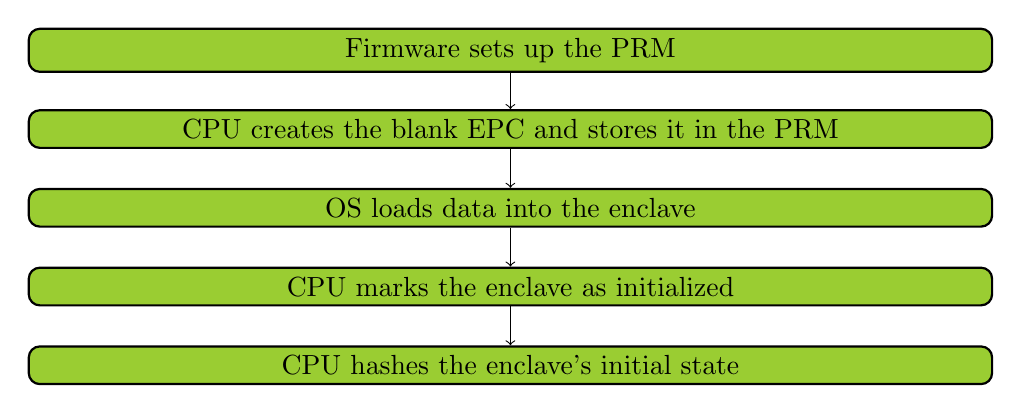
\begin{tikzpicture}[
    block/.style ={rectangle, draw=black, thick, fill=YellowGreen,
          text width=12cm, text centered, rounded corners},
    line/.style ={draw, ->}
]

\node[block] (s1) at (0,0) {Firmware sets up the PRM};
\node[block, below of = s1] (s3) {CPU creates the blank EPC and stores it in the PRM};
\node[block, below of = s3] (s5) {OS loads data into the enclave};
\node[block, below of = s5] (s10) {CPU marks the enclave as initialized};
\node[block, below of = s10] (s15) {CPU hashes the enclave’s initial state};

\path [line] (s1) -- (s3);
\path [line] (s3) -- (s5);
\path [line] (s5) -- (s10);
\path [line] (s10) -- (s15);

\end{tikzpicture}

\caption[Setting Up Intel SGX]{\textbf{Workflow for setting up an enclave.} It is important to note that the firmware which sets up the \gls{prm} and creates the \gls{epc} is vendor specific. It is highly probable that the firmware is based on the open source project TianoCore, an implementation of \gls{uefi} spearheaded by Intel in 2006 and now led by engineers from companies like Intel, Arm, Apple, and Red Hat.}
\label{fig:sgx-setup}
\end{figure}

\section{Executing SGX Enclave Code}
Execution flow can only move into an enclave via a special CPU instruction EENTER, much like switching from user mode to kernel mode. The actual execution happens in ``user mode'' also known as ``ring 3'' and takes advantage of address translation from the operating system or hypervisor. The benefit to this model is that the OS or hypervisor will quickly provide address translation lowering overhead. As Costan notes, ``the operating system and hypervisor are still in full control of the page tables and extended page tables (EPT), and each enclave's code uses the same address translation process and page tables as its host application. This minimizes the amount of changes required to add \gls{sgx} support to existing system software.'' \cite{Costan2016}. The downside is that code executing inside the enclave does not have access to system calls (syscall) or any other high privilege operations. This limits the types of operations that can be preformed inside an enclave. The code executing inside the enclave does have access to its entire address space which includes the ``host applicaion'' that caused the creation of the enclave.

The CPU executing the enclave code will perform an \gls{aex} whenever execution moves outside the enclave such as servicing an interrupt or during a page fault. The CPU state is saved inside the enclave memory metadata before exiting, ensuring that the CPU can securely restore the state of enclave execution. There are special machine mode CPU instructions that are used both in allocating \gls{epc} pages to the enclave as well as evicting those pages into untrusted DRAM. This facilitates code outside the enclave to operate on code within the enclave. \gls{sgx} uses cryptographic protections to assure the confidentiality, integrity and ``freshness'' \cite{Costan2016} of the evicted \gls{epc} pages while they are stored in untrusted memory. 

As mentioned the application that makes calls into an enclave or ``host application'' lives in the same address space as the enclave code and data. This has benefits in terms of application size variability, but may open the host application up to attack should the enclave code become compromised \cite{schwarz2019practical}.  \gls{sgx} allows enclaves to execute multiple threads through a \gls{tcs} which allows multiple logical cores to execute enclave code. Within the \gls{epc} metadata, reserved secure memory called the \gls{ssa} allows the threads to save their state when a context switch happens, like servicing an interrupt. In this way, Intel \gls{sgx} is able to allow a specific amount of code and data to remain protected while still allowing access to that data by code outside the trust boundary.

\section{Life Cycle of an SGX Enclave}

\begin{figure}[ht]
\makebox[\textwidth][c]{\begin{tikzpicture}[
	state/.style={draw, ellipse, text width=2cm, minimum height=1.4cm, align=center},
	arrow/.style={-latex'},
	label/.style={text width=3cm, align=center, font=\small}
]
\node[state] (v1) at (0,0) {non-existent};
\node[state] (v2) at (6,0) {not initialized};
\node[state, fill=CornflowerBlue!10!white] (v3) at (6,-4.5) {initialized};
\node[state, fill=CornflowerBlue!10!white] (v4) at (0,-4.5) {initialized\\(in use)};

\draw[arrow]  (v1) edge node[above, label] {ECREATE} (v2);
\draw[arrow]  (v2) edge node[right, label, align=left] {EINIT} (v3);
\draw[arrow]  (v2) edge[loop, looseness=5, in=330, out=30] node[right, label, align=left] {EADD\\EEXTEND} (v2);
\draw[arrow]  (v3) edge[loop, looseness=5, in=300, out=240] node[below, label] {page management instructions} (v3);
\draw[arrow]  (v3) edge[bend left=15] node[below, label] {EENTER\\ERESUME} (v4);
\draw[arrow]  (v4) edge[bend left=15] node[above, label] {EEXIT\\AEX} (v3);
\draw[arrow]  (v3) edge[bend right=15] node[below left, label, align=right, pos=0.7] {EREMOVE} (v1);
\draw[arrow]  (v4) edge[loop, looseness=5, in=300, out=240] node[below, label] {page management instructions} (v4);
\draw[arrow]  (v4) edge[loop, looseness=5, in=210, out=150] node[left, align=right] {EGETKEY\\EREPORT} (v4);
\end{tikzpicture}}
\caption[Intel SGX Enclave Lifecycle]{\textbf{Intel SGX enclave life cycle.} The enclave's memory is protected in states shaded blue. Note that in the enclave is not secure while in the uninitialized state as pages are being added or extended. Until a measurement is loaded into the MRENCLAVE register, code and data integrity can not be assured. The CPU will call AEX in order to service interrupts, and the state of the enclave will be saved in the \gls{ssa}. Reprinted as a simplified version from Costan's Figure 63 \cite{Costan2016}.\label{figure:sgx-enclave-life-cycle}}
\end{figure}

In order to understand the life cycle of an enclave, we must consider the specific x86 instructions used to create and manage these enclaves. Many of these instructions which create enclaves, extend pages, and remove enclaves operate in ``ring 0'', one of the most privileged modes. Whereas attestation, entering, and exiting the enclave can be done from ``ring 3'' the least privileged mode. The first of the privileged instructions in our life cycle is ECREATE which fills a protected data structure located inside the \gls{epc} with the size and hash of the enclave. This data structure, called the \gls{secs}, is used by the hardware and is not directly accessible to software. The system will then add pages to the \gls{epc} with the EADD instruction, and extend the \gls{epc} page \gls{measurement} with the EEXTEND instruction. When executing EADD and EEXTEND the system will ensure that the page's address range is within the Enclave Linear Range (ELRANGE). The EEXTEND instruction allows for the accumulation of a hash of all the pages in the \gls{epc}. This measurement can be used later for \gls{attestation} that the enclave has not been tampered with or changed in some way.

It is important to note that in its uninitialized state, none of the enclave code or data is encrypted. For example, any privileged driver running at ``ring 0'' can gain access to these data and structures. Enclaves must be initially built on a system that is known to be secure, such that the measurements taken are considered a ``gold standard'' with which to preform attestation on a local or remote machine at some later time. When the EINIT instruction is called, the enclave is considered fully built, the measurement is locked down, and ``ring 3'' (user) applications can now enter the enclave and attest that it contains the code and data that the developer intended. 

EBLOCK, ETRACK, EWB, and ELOAD\footnote{Actually, two load commands, ELDB and ELDU both load into memory a previously evicted page, with ELDB for blocked and ELDU for unblocked. Pages may be blocked when being prepared for eviction. All future accesses to blocked pages will result in a page fault.} are paging instructions run with ``ring 0'' privileges. The goal is to allow the paging of secure pages into and out of main memory while ensuring the confidentiality and integrity of those pages. Information stored inside the \gls{epc} called the \gls{pcmd} keeps track of the identity of the enclave the page belongs to and a pointer to an access rights structure. There is also a \gls{va} which is used to store the version numbers of pages evicted from the \gls{epc}. These versioned and access controlled pages are therefore hardware protected, and any change to the versioning, access rights, or origins of the page will result in a page fault. It is possible to have 2 instances of the same enclave, however pages cannot be swapped between them, and the hashes of these pages will not be the same.

Once an application has requested that ``ring 0'' components build the enclave and EENTER is called, the enclave may begin execution. The hardware is responsible for saving (AEX) and restoring (ERESUME) the architectural state of execution should any external events like interrupts or exceptions cause execution to leave the enclave. The EGETKEY and EREPORT instructions operate in user mode (``ring 3'') and seal data based on the key the developer provides. Using these two instructions \gls{sgx} applications operating in ``ring 3'' are able to preform local attestation of the enclave, perhaps the most vital function of any \gls{tee}. Finally, once the enclave is no longer needed, the system will call EEXIT, and a synchronous enclave exit will occur. As Costan notes, ``EEXIT does not modify most registers, so enclave authors must make sure to clear any secrets stored in the processor’s registers before returning control to the host process.'' \cite{Costan2016}.

\section{Attestation with Intel SGX}
Software attestation of enclaves is required to ensure the integrity of the enclave. This attestation can happen locally between two enclaves on the same platform or remotely between two different platforms. As previously noted, the measurement of the enclave includes a SHA-256 hash of the enclave's attributes as well as the content, position, and access rights of its pages. This measurement is stored in a register called MRENCLAVE which represents the enclave's \gls{tcb}. The EREPORT instruction is used to generate a signed report of this \gls{tcb} and the EGETKEY instruction then retrieves the key used to validate said report. Local attestation of enclaves can be done using symmetric encryption as the hardware can ensure the integrity of the single key being used to verify the MRENCLAVE value. Remote attestation must be done using asymmetric encryption (both a public and private key) and requires the remote \gls{sgx} enabled platform to query an Intel attestation server.

\begin{figure}[ht]
\centering
\makebox[\linewidth]{
\begin{tikzpicture}[scale=0.8, transform shape,
nodes={text width=3cm, align=center, minimum height=2.5cm},
numarr/.style={draw=none,anchor=center,yshift=.25cm,pos=0.5},
numarrv/.style={draw=none,anchor=center,xshift=.25cm,pos=0.5},
small/.style={font=\small}]

% nodes
\node [draw] (v1) at (-9,9) {Challenger};
\node [draw] (v5) at (-9,5) {Attestation Verification};
\node [draw] (v2) at (-3.5,9) {Application};
\node [draw] (v3) at (3.5,9) {\textbf{Application Enclave}\\User Data \faKey};
\node [draw] (v4) at (-3.5,5) {\textbf{Quoting Enclave}\\ Attestation Key \faKey};
\node [] at (-9,11.5) {Remote Platform};
\node [] at (.5,11.5) {User Platform};

% edges
\draw [-latex'] ([yshift=.5cm]v1.east) -- ([yshift=.5cm]v2.west) node [numarr] {1};
\draw [-latex'] ([yshift=-.5cm]v2.west) -- ([yshift=-.5cm]v1.east) node [numarr] {6};
\draw [-latex'] ([yshift=.5cm]v2.east) -- ([yshift=.5cm]v3.west) node [numarr] {2};
\draw [-latex'] ([yshift=-.5cm]v3.west) -- ([yshift=-.5cm]v2.east) node [numarr] {3};
\draw [-latex'] ([xshift=-.75cm]v2.south) -- ([xshift=-.75cm]v4.north) node [numarrv] {4};
\draw [-latex'] ([xshift=.75cm]v4.north) -- ([xshift=.75cm]v2.south) node [numarrv] {5};
\draw [latex'-latex'] (v1) -- (v5) node [numarrv] {7};

% fits
\begin{scope}[on background layer]
  \draw [dotted] (-11,12) rectangle (-7,3);
  \draw [dotted, fill=CornflowerBlue!10!white] (-6,12) rectangle (6.5,3);
\end{scope}
\end{tikzpicture}
}

\caption[Intel SGX Attestation]{\textbf{Local and remote attestation of an Intel SGX enclave.} A remote challenger may request that an application provide attestation. The application must then request a report from the enclave and locally verify that against a quoting enclave. The quoting enclave will use the remote along with asymmetric keys to produce a remote attestation ``quote'' to be returned to the challenger. The challenger may then use some verification service to check the validity of the quote. This figure was reproduced from Figure 1 \cite{johnson2016intel}.}
\label{fig:sgx-attest}
\end{figure}

Local attestation can be used by enclaves running on the same platform and will provide assurance as to the identity of the enclaves. The local enclave which attests to the reporting enclave is called the ``Quoting Enclave'' \cite{johnson2016intel}. Figure \ref{fig:sgx-attest} provides a high level overview of the attestation process including both local and remote attestation. On today's complex and connected systems, local attestation alone is not enough to assure that the platform and enclave are genuine \gls{sgx} enclaves \cite{knauth2018integrating}. Remote attestation requires asymmetric keys as well as a remote server with which to verify the quote of an enclave.

Intel platforms include two statistically unique ``root keys'' which provide assurance that the system is indeed a genuine Intel \gls{sgx} platform. These include the Root Provisioning Key and the Root Seal Key \cite{johnson2016intel} which are stored in hardware fuses. Intel also provides a more advanced form of asymmetric encryption called \gls{epid}. This is essentially a group signature where the system can attest to a message being signed by a member of the group without divulging the identify of the signer. The signature algorithm is nothing new \cite{brickell2007enhanced} and has been included in the ISO/IEC 20008 and 20009 standards. \gls{epid} includes several revocation schemes which allow keys to be revoked based on checks performed by the verifier and/or issuer. The Intel Attestation Service (IAS) will take submission of quotes provided, verify the validity of the signatures, and verify that they have not been revoked.

In this chapter, we have briefly described Intel \glsreset{sgx}\gls{sgx} from the initial setup of the enclave through to the remote attestation of that enclave's contents. This system is by far the most complex of the three we will examine in this thesis. We have only covered the properties that are necessary to understand if we are to appropriately apply our method of comparison. Depending on the use case, a much more in depth knowledge of \gls{sgx} may be required. However, we hope to show that even with this rudimentary understanding, one can still apply rigorous method to analysing features of a \gls{tee}. Next, we will cover Arm's framework for building \glspl{tee} called TrustZone, as well as the reference implementations of their firmware: \gls{tfa} and \gls{optee}.